\documentclass{article} % For LaTeX2e
\usepackage{iclr2022_conference,times}
% Optional math commands from https://github.com/goodfeli/dlbook_notation.
%%%%% NEW MATH DEFINITIONS %%%%%

\usepackage{amsmath,amsfonts,bm}

% Mark sections of captions for referring to divisions of figures
\newcommand{\figleft}{{\em (Left)}}
\newcommand{\figcenter}{{\em (Center)}}
\newcommand{\figright}{{\em (Right)}}
\newcommand{\figtop}{{\em (Top)}}
\newcommand{\figbottom}{{\em (Bottom)}}
\newcommand{\captiona}{{\em (a)}}
\newcommand{\captionb}{{\em (b)}}
\newcommand{\captionc}{{\em (c)}}
\newcommand{\captiond}{{\em (d)}}

% Highlight a newly defined term
\newcommand{\newterm}[1]{{\bf #1}}


% Figure reference, lower-case.
\def\figref#1{figure~\ref{#1}}
% Figure reference, capital. For start of sentence
\def\Figref#1{Figure~\ref{#1}}
\def\twofigref#1#2{figures \ref{#1} and \ref{#2}}
\def\quadfigref#1#2#3#4{figures \ref{#1}, \ref{#2}, \ref{#3} and \ref{#4}}
% Section reference, lower-case.
\def\secref#1{section~\ref{#1}}
% Section reference, capital.
\def\Secref#1{Section~\ref{#1}}
% Reference to two sections.
\def\twosecrefs#1#2{sections \ref{#1} and \ref{#2}}
% Reference to three sections.
\def\secrefs#1#2#3{sections \ref{#1}, \ref{#2} and \ref{#3}}
% Reference to an equation, lower-case.
\def\eqref#1{equation~\ref{#1}}
% Reference to an equation, upper case
\def\Eqref#1{Equation~\ref{#1}}
% A raw reference to an equation---avoid using if possible
\def\plaineqref#1{\ref{#1}}
% Reference to a chapter, lower-case.
\def\chapref#1{chapter~\ref{#1}}
% Reference to an equation, upper case.
\def\Chapref#1{Chapter~\ref{#1}}
% Reference to a range of chapters
\def\rangechapref#1#2{chapters\ref{#1}--\ref{#2}}
% Reference to an algorithm, lower-case.
\def\algref#1{algorithm~\ref{#1}}
% Reference to an algorithm, upper case.
\def\Algref#1{Algorithm~\ref{#1}}
\def\twoalgref#1#2{algorithms \ref{#1} and \ref{#2}}
\def\Twoalgref#1#2{Algorithms \ref{#1} and \ref{#2}}
% Reference to a part, lower case
\def\partref#1{part~\ref{#1}}
% Reference to a part, upper case
\def\Partref#1{Part~\ref{#1}}
\def\twopartref#1#2{parts \ref{#1} and \ref{#2}}

\def\ceil#1{\lceil #1 \rceil}
\def\floor#1{\lfloor #1 \rfloor}
\def\1{\bm{1}}
\newcommand{\train}{\mathcal{D}}
\newcommand{\valid}{\mathcal{D_{\mathrm{valid}}}}
\newcommand{\test}{\mathcal{D_{\mathrm{test}}}}

\def\eps{{\epsilon}}


% Random variables
\def\reta{{\textnormal{$\eta$}}}
\def\ra{{\textnormal{a}}}
\def\rb{{\textnormal{b}}}
\def\rc{{\textnormal{c}}}
\def\rd{{\textnormal{d}}}
\def\re{{\textnormal{e}}}
\def\rf{{\textnormal{f}}}
\def\rg{{\textnormal{g}}}
\def\rh{{\textnormal{h}}}
\def\ri{{\textnormal{i}}}
\def\rj{{\textnormal{j}}}
\def\rk{{\textnormal{k}}}
\def\rl{{\textnormal{l}}}
% rm is already a command, just don't name any random variables m
\def\rn{{\textnormal{n}}}
\def\ro{{\textnormal{o}}}
\def\rp{{\textnormal{p}}}
\def\rq{{\textnormal{q}}}
\def\rr{{\textnormal{r}}}
\def\rs{{\textnormal{s}}}
\def\rt{{\textnormal{t}}}
\def\ru{{\textnormal{u}}}
\def\rv{{\textnormal{v}}}
\def\rw{{\textnormal{w}}}
\def\rx{{\textnormal{x}}}
\def\ry{{\textnormal{y}}}
\def\rz{{\textnormal{z}}}

% Random vectors
\def\rvepsilon{{\mathbf{\epsilon}}}
\def\rvtheta{{\mathbf{\theta}}}
\def\rva{{\mathbf{a}}}
\def\rvb{{\mathbf{b}}}
\def\rvc{{\mathbf{c}}}
\def\rvd{{\mathbf{d}}}
\def\rve{{\mathbf{e}}}
\def\rvf{{\mathbf{f}}}
\def\rvg{{\mathbf{g}}}
\def\rvh{{\mathbf{h}}}
\def\rvu{{\mathbf{i}}}
\def\rvj{{\mathbf{j}}}
\def\rvk{{\mathbf{k}}}
\def\rvl{{\mathbf{l}}}
\def\rvm{{\mathbf{m}}}
\def\rvn{{\mathbf{n}}}
\def\rvo{{\mathbf{o}}}
\def\rvp{{\mathbf{p}}}
\def\rvq{{\mathbf{q}}}
\def\rvr{{\mathbf{r}}}
\def\rvs{{\mathbf{s}}}
\def\rvt{{\mathbf{t}}}
\def\rvu{{\mathbf{u}}}
\def\rvv{{\mathbf{v}}}
\def\rvw{{\mathbf{w}}}
\def\rvx{{\mathbf{x}}}
\def\rvy{{\mathbf{y}}}
\def\rvz{{\mathbf{z}}}

% Elements of random vectors
\def\erva{{\textnormal{a}}}
\def\ervb{{\textnormal{b}}}
\def\ervc{{\textnormal{c}}}
\def\ervd{{\textnormal{d}}}
\def\erve{{\textnormal{e}}}
\def\ervf{{\textnormal{f}}}
\def\ervg{{\textnormal{g}}}
\def\ervh{{\textnormal{h}}}
\def\ervi{{\textnormal{i}}}
\def\ervj{{\textnormal{j}}}
\def\ervk{{\textnormal{k}}}
\def\ervl{{\textnormal{l}}}
\def\ervm{{\textnormal{m}}}
\def\ervn{{\textnormal{n}}}
\def\ervo{{\textnormal{o}}}
\def\ervp{{\textnormal{p}}}
\def\ervq{{\textnormal{q}}}
\def\ervr{{\textnormal{r}}}
\def\ervs{{\textnormal{s}}}
\def\ervt{{\textnormal{t}}}
\def\ervu{{\textnormal{u}}}
\def\ervv{{\textnormal{v}}}
\def\ervw{{\textnormal{w}}}
\def\ervx{{\textnormal{x}}}
\def\ervy{{\textnormal{y}}}
\def\ervz{{\textnormal{z}}}

% Random matrices
\def\rmA{{\mathbf{A}}}
\def\rmB{{\mathbf{B}}}
\def\rmC{{\mathbf{C}}}
\def\rmD{{\mathbf{D}}}
\def\rmE{{\mathbf{E}}}
\def\rmF{{\mathbf{F}}}
\def\rmG{{\mathbf{G}}}
\def\rmH{{\mathbf{H}}}
\def\rmI{{\mathbf{I}}}
\def\rmJ{{\mathbf{J}}}
\def\rmK{{\mathbf{K}}}
\def\rmL{{\mathbf{L}}}
\def\rmM{{\mathbf{M}}}
\def\rmN{{\mathbf{N}}}
\def\rmO{{\mathbf{O}}}
\def\rmP{{\mathbf{P}}}
\def\rmQ{{\mathbf{Q}}}
\def\rmR{{\mathbf{R}}}
\def\rmS{{\mathbf{S}}}
\def\rmT{{\mathbf{T}}}
\def\rmU{{\mathbf{U}}}
\def\rmV{{\mathbf{V}}}
\def\rmW{{\mathbf{W}}}
\def\rmX{{\mathbf{X}}}
\def\rmY{{\mathbf{Y}}}
\def\rmZ{{\mathbf{Z}}}

% Elements of random matrices
\def\ermA{{\textnormal{A}}}
\def\ermB{{\textnormal{B}}}
\def\ermC{{\textnormal{C}}}
\def\ermD{{\textnormal{D}}}
\def\ermE{{\textnormal{E}}}
\def\ermF{{\textnormal{F}}}
\def\ermG{{\textnormal{G}}}
\def\ermH{{\textnormal{H}}}
\def\ermI{{\textnormal{I}}}
\def\ermJ{{\textnormal{J}}}
\def\ermK{{\textnormal{K}}}
\def\ermL{{\textnormal{L}}}
\def\ermM{{\textnormal{M}}}
\def\ermN{{\textnormal{N}}}
\def\ermO{{\textnormal{O}}}
\def\ermP{{\textnormal{P}}}
\def\ermQ{{\textnormal{Q}}}
\def\ermR{{\textnormal{R}}}
\def\ermS{{\textnormal{S}}}
\def\ermT{{\textnormal{T}}}
\def\ermU{{\textnormal{U}}}
\def\ermV{{\textnormal{V}}}
\def\ermW{{\textnormal{W}}}
\def\ermX{{\textnormal{X}}}
\def\ermY{{\textnormal{Y}}}
\def\ermZ{{\textnormal{Z}}}

% Vectors
\def\vzero{{\bm{0}}}
\def\vone{{\bm{1}}}
\def\vmu{{\bm{\mu}}}
\def\vtheta{{\bm{\theta}}}
\def\va{{\bm{a}}}
\def\vb{{\bm{b}}}
\def\vc{{\bm{c}}}
\def\vd{{\bm{d}}}
\def\ve{{\bm{e}}}
\def\vf{{\bm{f}}}
\def\vg{{\bm{g}}}
\def\vh{{\bm{h}}}
\def\vi{{\bm{i}}}
\def\vj{{\bm{j}}}
\def\vk{{\bm{k}}}
\def\vl{{\bm{l}}}
\def\vm{{\bm{m}}}
\def\vn{{\bm{n}}}
\def\vo{{\bm{o}}}
\def\vp{{\bm{p}}}
\def\vq{{\bm{q}}}
\def\vr{{\bm{r}}}
\def\vs{{\bm{s}}}
\def\vt{{\bm{t}}}
\def\vu{{\bm{u}}}
\def\vv{{\bm{v}}}
\def\vw{{\bm{w}}}
\def\vx{{\bm{x}}}
\def\vy{{\bm{y}}}
\def\vz{{\bm{z}}}

% Elements of vectors
\def\evalpha{{\alpha}}
\def\evbeta{{\beta}}
\def\evepsilon{{\epsilon}}
\def\evlambda{{\lambda}}
\def\evomega{{\omega}}
\def\evmu{{\mu}}
\def\evpsi{{\psi}}
\def\evsigma{{\sigma}}
\def\evtheta{{\theta}}
\def\eva{{a}}
\def\evb{{b}}
\def\evc{{c}}
\def\evd{{d}}
\def\eve{{e}}
\def\evf{{f}}
\def\evg{{g}}
\def\evh{{h}}
\def\evi{{i}}
\def\evj{{j}}
\def\evk{{k}}
\def\evl{{l}}
\def\evm{{m}}
\def\evn{{n}}
\def\evo{{o}}
\def\evp{{p}}
\def\evq{{q}}
\def\evr{{r}}
\def\evs{{s}}
\def\evt{{t}}
\def\evu{{u}}
\def\evv{{v}}
\def\evw{{w}}
\def\evx{{x}}
\def\evy{{y}}
\def\evz{{z}}

% Matrix
\def\mA{{\bm{A}}}
\def\mB{{\bm{B}}}
\def\mC{{\bm{C}}}
\def\mD{{\bm{D}}}
\def\mE{{\bm{E}}}
\def\mF{{\bm{F}}}
\def\mG{{\bm{G}}}
\def\mH{{\bm{H}}}
\def\mI{{\bm{I}}}
\def\mJ{{\bm{J}}}
\def\mK{{\bm{K}}}
\def\mL{{\bm{L}}}
\def\mM{{\bm{M}}}
\def\mN{{\bm{N}}}
\def\mO{{\bm{O}}}
\def\mP{{\bm{P}}}
\def\mQ{{\bm{Q}}}
\def\mR{{\bm{R}}}
\def\mS{{\bm{S}}}
\def\mT{{\bm{T}}}
\def\mU{{\bm{U}}}
\def\mV{{\bm{V}}}
\def\mW{{\bm{W}}}
\def\mX{{\bm{X}}}
\def\mY{{\bm{Y}}}
\def\mZ{{\bm{Z}}}
\def\mBeta{{\bm{\beta}}}
\def\mPhi{{\bm{\Phi}}}
\def\mLambda{{\bm{\Lambda}}}
\def\mSigma{{\bm{\Sigma}}}

% Tensor
\DeclareMathAlphabet{\mathsfit}{\encodingdefault}{\sfdefault}{m}{sl}
\SetMathAlphabet{\mathsfit}{bold}{\encodingdefault}{\sfdefault}{bx}{n}
\newcommand{\tens}[1]{\bm{\mathsfit{#1}}}
\def\tA{{\tens{A}}}
\def\tB{{\tens{B}}}
\def\tC{{\tens{C}}}
\def\tD{{\tens{D}}}
\def\tE{{\tens{E}}}
\def\tF{{\tens{F}}}
\def\tG{{\tens{G}}}
\def\tH{{\tens{H}}}
\def\tI{{\tens{I}}}
\def\tJ{{\tens{J}}}
\def\tK{{\tens{K}}}
\def\tL{{\tens{L}}}
\def\tM{{\tens{M}}}
\def\tN{{\tens{N}}}
\def\tO{{\tens{O}}}
\def\tP{{\tens{P}}}
\def\tQ{{\tens{Q}}}
\def\tR{{\tens{R}}}
\def\tS{{\tens{S}}}
\def\tT{{\tens{T}}}
\def\tU{{\tens{U}}}
\def\tV{{\tens{V}}}
\def\tW{{\tens{W}}}
\def\tX{{\tens{X}}}
\def\tY{{\tens{Y}}}
\def\tZ{{\tens{Z}}}


% Graph
\def\gA{{\mathcal{A}}}
\def\gB{{\mathcal{B}}}
\def\gC{{\mathcal{C}}}
\def\gD{{\mathcal{D}}}
\def\gE{{\mathcal{E}}}
\def\gF{{\mathcal{F}}}
\def\gG{{\mathcal{G}}}
\def\gH{{\mathcal{H}}}
\def\gI{{\mathcal{I}}}
\def\gJ{{\mathcal{J}}}
\def\gK{{\mathcal{K}}}
\def\gL{{\mathcal{L}}}
\def\gM{{\mathcal{M}}}
\def\gN{{\mathcal{N}}}
\def\gO{{\mathcal{O}}}
\def\gP{{\mathcal{P}}}
\def\gQ{{\mathcal{Q}}}
\def\gR{{\mathcal{R}}}
\def\gS{{\mathcal{S}}}
\def\gT{{\mathcal{T}}}
\def\gU{{\mathcal{U}}}
\def\gV{{\mathcal{V}}}
\def\gW{{\mathcal{W}}}
\def\gX{{\mathcal{X}}}
\def\gY{{\mathcal{Y}}}
\def\gZ{{\mathcal{Z}}}

% Sets
\def\sA{{\mathbb{A}}}
\def\sB{{\mathbb{B}}}
\def\sC{{\mathbb{C}}}
\def\sD{{\mathbb{D}}}
% Don't use a set called E, because this would be the same as our symbol
% for expectation.
\def\sF{{\mathbb{F}}}
\def\sG{{\mathbb{G}}}
\def\sH{{\mathbb{H}}}
\def\sI{{\mathbb{I}}}
\def\sJ{{\mathbb{J}}}
\def\sK{{\mathbb{K}}}
\def\sL{{\mathbb{L}}}
\def\sM{{\mathbb{M}}}
\def\sN{{\mathbb{N}}}
\def\sO{{\mathbb{O}}}
\def\sP{{\mathbb{P}}}
\def\sQ{{\mathbb{Q}}}
\def\sR{{\mathbb{R}}}
\def\sS{{\mathbb{S}}}
\def\sT{{\mathbb{T}}}
\def\sU{{\mathbb{U}}}
\def\sV{{\mathbb{V}}}
\def\sW{{\mathbb{W}}}
\def\sX{{\mathbb{X}}}
\def\sY{{\mathbb{Y}}}
\def\sZ{{\mathbb{Z}}}

% Entries of a matrix
\def\emLambda{{\Lambda}}
\def\emA{{A}}
\def\emB{{B}}
\def\emC{{C}}
\def\emD{{D}}
\def\emE{{E}}
\def\emF{{F}}
\def\emG{{G}}
\def\emH{{H}}
\def\emI{{I}}
\def\emJ{{J}}
\def\emK{{K}}
\def\emL{{L}}
\def\emM{{M}}
\def\emN{{N}}
\def\emO{{O}}
\def\emP{{P}}
\def\emQ{{Q}}
\def\emR{{R}}
\def\emS{{S}}
\def\emT{{T}}
\def\emU{{U}}
\def\emV{{V}}
\def\emW{{W}}
\def\emX{{X}}
\def\emY{{Y}}
\def\emZ{{Z}}
\def\emSigma{{\Sigma}}

% entries of a tensor
% Same font as tensor, without \bm wrapper
\newcommand{\etens}[1]{\mathsfit{#1}}
\def\etLambda{{\etens{\Lambda}}}
\def\etA{{\etens{A}}}
\def\etB{{\etens{B}}}
\def\etC{{\etens{C}}}
\def\etD{{\etens{D}}}
\def\etE{{\etens{E}}}
\def\etF{{\etens{F}}}
\def\etG{{\etens{G}}}
\def\etH{{\etens{H}}}
\def\etI{{\etens{I}}}
\def\etJ{{\etens{J}}}
\def\etK{{\etens{K}}}
\def\etL{{\etens{L}}}
\def\etM{{\etens{M}}}
\def\etN{{\etens{N}}}
\def\etO{{\etens{O}}}
\def\etP{{\etens{P}}}
\def\etQ{{\etens{Q}}}
\def\etR{{\etens{R}}}
\def\etS{{\etens{S}}}
\def\etT{{\etens{T}}}
\def\etU{{\etens{U}}}
\def\etV{{\etens{V}}}
\def\etW{{\etens{W}}}
\def\etX{{\etens{X}}}
\def\etY{{\etens{Y}}}
\def\etZ{{\etens{Z}}}

% The true underlying data generating distribution
\newcommand{\pdata}{p_{\rm{data}}}
% The empirical distribution defined by the training set
\newcommand{\ptrain}{\hat{p}_{\rm{data}}}
\newcommand{\Ptrain}{\hat{P}_{\rm{data}}}
% The model distribution
\newcommand{\pmodel}{p_{\rm{model}}}
\newcommand{\Pmodel}{P_{\rm{model}}}
\newcommand{\ptildemodel}{\tilde{p}_{\rm{model}}}
% Stochastic autoencoder distributions
\newcommand{\pencode}{p_{\rm{encoder}}}
\newcommand{\pdecode}{p_{\rm{decoder}}}
\newcommand{\precons}{p_{\rm{reconstruct}}}

\newcommand{\laplace}{\mathrm{Laplace}} % Laplace distribution

\newcommand{\E}{\mathbb{E}}
\newcommand{\Ls}{\mathcal{L}}
\newcommand{\R}{\mathbb{R}}
\newcommand{\emp}{\tilde{p}}
\newcommand{\lr}{\alpha}
\newcommand{\reg}{\lambda}
\newcommand{\rect}{\mathrm{rectifier}}
\newcommand{\softmax}{\mathrm{softmax}}
\newcommand{\sigmoid}{\sigma}
\newcommand{\softplus}{\zeta}
\newcommand{\KL}{D_{\mathrm{KL}}}
\newcommand{\Var}{\mathrm{Var}}
\newcommand{\standarderror}{\mathrm{SE}}
\newcommand{\Cov}{\mathrm{Cov}}
% Wolfram Mathworld says $L^2$ is for function spaces and $\ell^2$ is for vectors
% But then they seem to use $L^2$ for vectors throughout the site, and so does
% wikipedia.
\newcommand{\normlzero}{L^0}
\newcommand{\normlone}{L^1}
\newcommand{\normltwo}{L^2}
\newcommand{\normlp}{L^p}
\newcommand{\normmax}{L^\infty}

\newcommand{\parents}{Pa} % See usage in notation.tex. Chosen to match Daphne's book.

\DeclareMathOperator*{\argmax}{arg\,max}
\DeclareMathOperator*{\argmin}{arg\,min}

\DeclareMathOperator{\sign}{sign}
\DeclareMathOperator{\Tr}{Tr}
\let\ab\allowbreak


%######## APS360: Uncomment your submission name
%\newcommand{\apsname}{Project Proposal}
%\newcommand{\apsname}{Progress Report}
\newcommand{\apsname}{Final Report}

%######## APS360: Put your Group Number here
\newcommand{\gpnumber}{20}

\usepackage{hyperref}
\usepackage{url}
\usepackage{graphicx}
\usepackage{multicol}
\usepackage{placeins}

%######## APS360: Put your project Title here
\title{Poetry Through Propogation,\ Generating Haikus With Deep Learning Recurrent Neural Networks}


%######## APS360: Put your names, student IDs and Emails here
\author{Evan Banerjee  \\
Student\# 1009682309\\
\texttt{evan.banerjee@mail.utoronto.ca} \\
\And
Diego Ciudad Real Escalante  \\
Student\# 1009345308 \\
\texttt{diego.ciudadrealescalante@mail.utoronto.ca} \\
\AND
Noah Monti  \\
Student\# 1009452398 \\
\texttt{noah.monti@mail.utoronto.ca} \\
\And
Ji Hong Sayo \\
Student\# 1007314728 \\
\texttt{ji.sayo@mail.utoronto.ca} \\
\AND
}

% The \author macro works with any number of authors. There are two commands
% used to separate the names and addresses of multiple authors: \And and \AND.
%
% Using \And between authors leaves it to \LaTeX{} to determine where to break
% the lines. Using \AND forces a linebreak at that point. So, if \LaTeX{}
% puts 3 of 4 authors names on the first line, and the last on the second
% line, try using \AND instead of \And before the third author name.

\newcommand{\fix}{\marginpar{FIX}}
\newcommand{\new}{\marginpar{NEW}}

\iclrfinalcopy 
%######## APS360: Document starts here
\begin{document}


\maketitle

\begin{abstract}
  This is our final report for the APS360 Final Project.
  %######## APS360: Do not change the next line. This shows your Main body page count.
  Total Pages: \pageref{last_page}
\end{abstract}

\section{Introduction}

“Genuine poetry can communicate before it is understood” —T.S. Eliot

In this project we are working to build a deep learning model to generate short poems of various topics.
Our model is a haiku generator which can be prompted with the first line of a haiku and generate the content of subsequent lines, built on a gated recurrent unit (GRU) architecture.
Poetry has long been regarded as a deep expression of emotion and human experience. Given that the model we construct will possess neither emotions nor intuition, we are interested to see whether our construction will be able to imitate human poetry, and if so to what degree. If the model is capable of producing compelling poems as output, this would contradict the idea that poetry requires emotion to produce, with implications for our understanding of the nature of creative work in general.

\begin{figure}[h]
  \begin{center}
  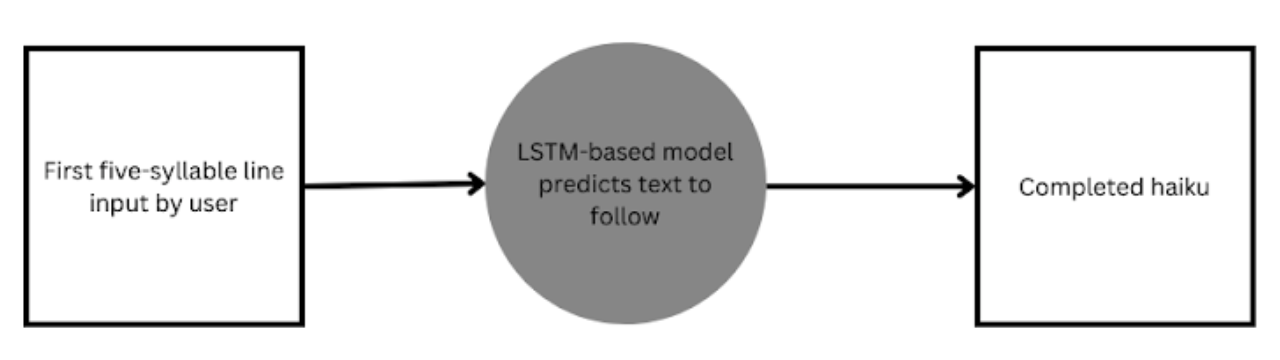
\includegraphics[width=1\textwidth]{Figs/pipeline.png}
  \end{center}
  \caption{Basic Model Pipeline}
  \label{fig:Basic Model Pipeline}
\end{figure}

Several ML approaches can be taken to text-generation. For instance, we compare our model to markov chains as a baseline. However, deep learning offers advantages that other statistical approaches cannot. As compared to simpler statistical models, neural nets can learn more abstract and general characteristics in the poems used for training. Given that a hallmark of good poetry is abstraction and unity around a sustaining theme, we believe deep learning is uniquely well-suited for the problem of poetry generation. 



\section{Illustriaton}
The high-level description of the model can be seen below in \ref{fig:model_diagram} .
The model consists of Gated Recurrent Unit that is trained on poems sourced from the web.
These poems also build up the dictionary of words used by the model to generate haikus.
Finally, the diagram also shows the expected usage of this model.
A user would prompt the model with the starting words of a poem, press enter,
and the model would generate a haiku with the prompt as its starting point.



\begin{figure}[h]
  \begin{center}
  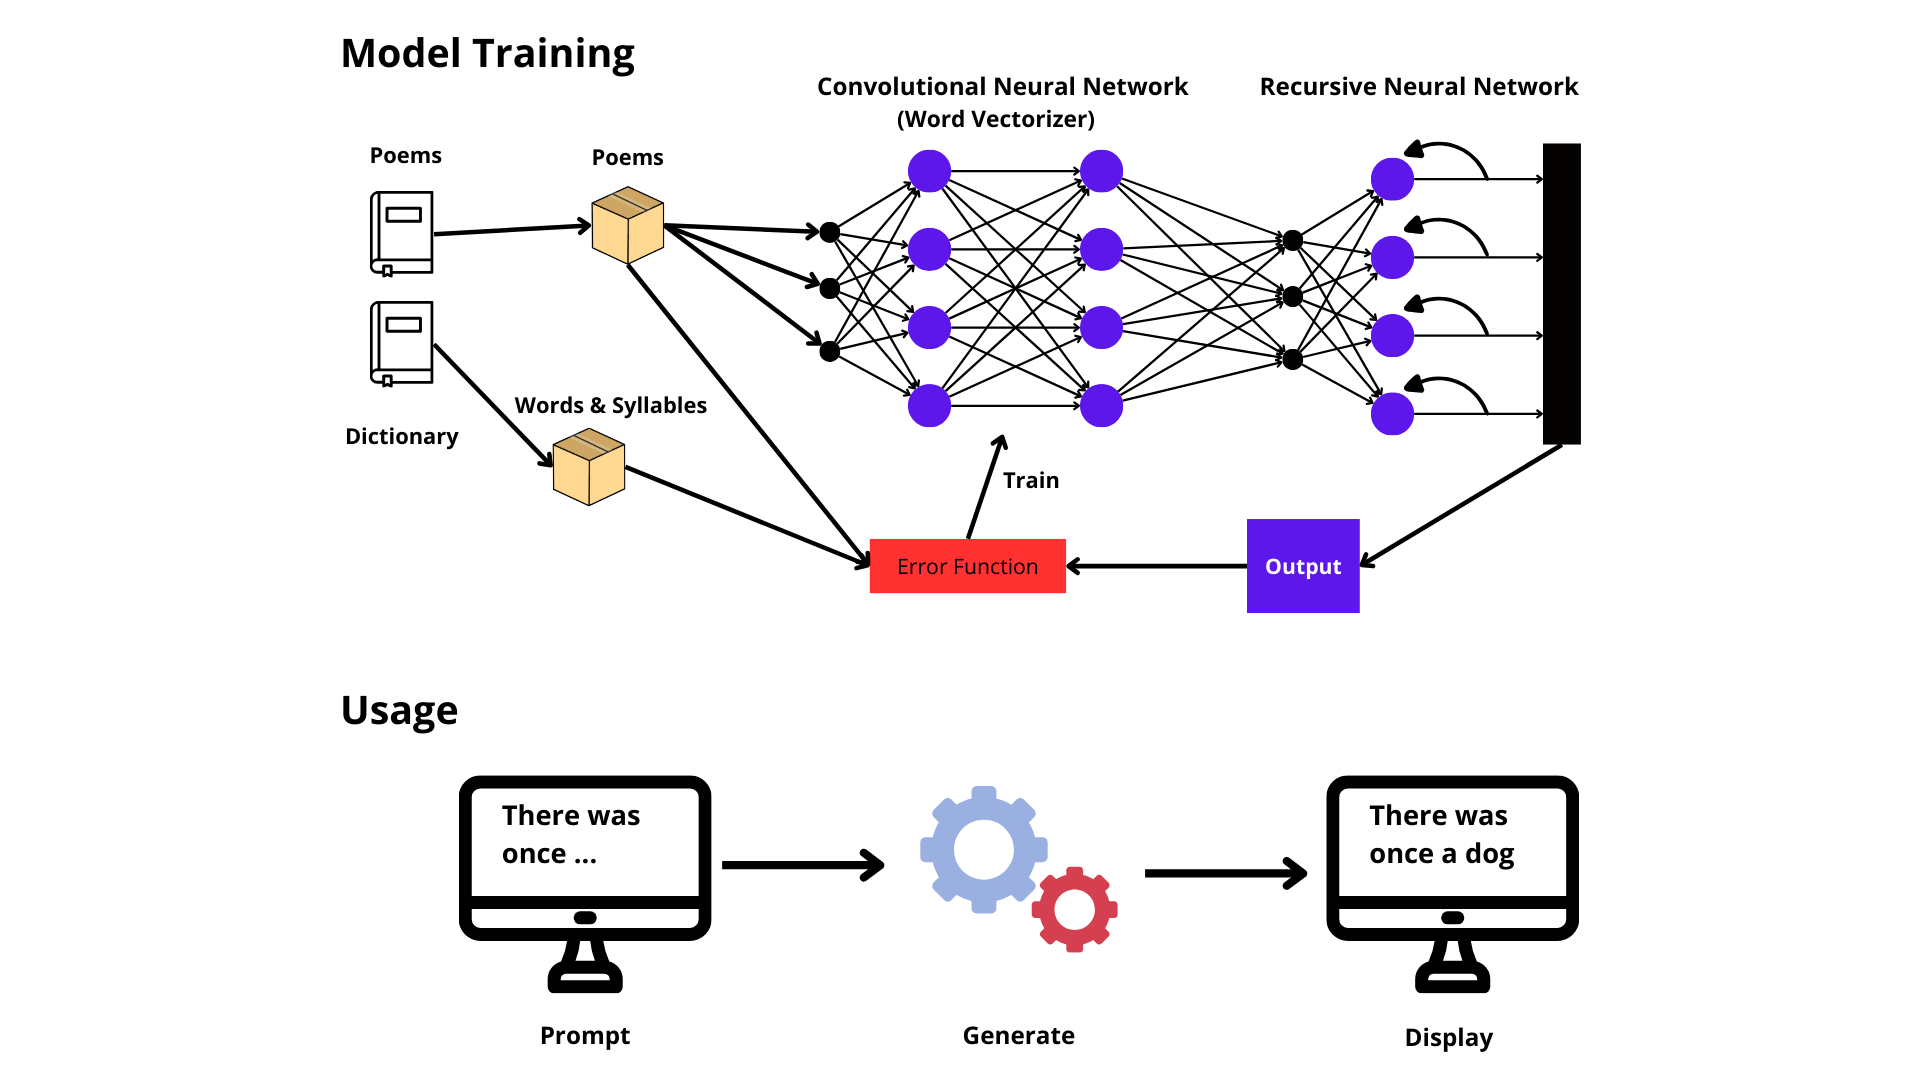
\includegraphics[width=1\textwidth]{Figs/model_diagram.png}
  \end{center}
  \caption{Top-Level Model Description}
  \label{fig:model_diagram}
\end{figure}

\section{Background}
Previous poetry generation models utilized Recurrent Neural Networks (RNN) with some form of memory limiting to generate poems off a large dataset.\\\\
One model, created by researchers at the University of Saarland, utilized encoder decoder systems, as well as long short-term memory (LSTM) and Gated Recurrent Units (GRU) to address vanishing gradients, \citep{novikovaenglish}.\\\\
Another model, developed at the University of Edinburgh utilized multiple neural networks chained together, with a convolutional neural network (CNN) for encoding, one RNN for creating hidden context parameters,
and another RNN with a separate weight vector for modifying the final output \citep{zhang2014chinese}.
The output of this model was particularly compelling, with human ratings for the generated poems being over 75\% of the ratings given to human written poems.\\\\
Another model, built at City, University of London, used syllables as the inputs and outputs of their RNN instead of words \citep{lewis2021syllable}.
This model’s poems were incredibly convincing, with 56\% of polled individuals believing the AI generated poems were written by humans.\\\\
When focusing specifically on haikus, even a relatively basic model built by students at Stanford University was able to score well \citep{haikugeneration}. 
For this model human evaluators gave the AI generated haikus an average quality score that was over 80\% of the average score given to human poems. This model only used a single RNN with LSTM. 
Granted, the evaluations were only done by 8 individuals, but the strength of RNNs for this kind of task is evident.\\\\
Finally, a model presented at the 13th conference on language resources and evaluation found a large degree of success in constraining the output of neural networks to generate poems \citep{popescu2022constrained}.
This model forced the AI to repeatedly output lines of a poem until certain syntax requirements were met.
It also enabled the user to specify emotional tone by encoding category preferences (happy, sad, etc.) into a weighted vector that was then used after generating a line to swap out words that didn’t fit the categories well with words that did.\\\\
This was most effectively done when words were chosen based on word frequency from other poems that fit the specified category. 
This model also utilized a softmax function that truncates the least likely words from the sample space during generation, increasing the probability of likely words and drastically improving output.\\\\
Each one of these model's utilized different techniques. Whether the differences were in the way they encoded and decoded the inputs and outputs, or the or the specific method they used to manage hidden states. Whether they used syllables as the their input output token, or whether they used words. Whether they forced the model to regenerate lines that didn't fit certain syntax requirements, used algorithms to swap out words after generating the lines, or simply left the lines as is. Each model had their own unique way of addressing the somewhat existential task of creating poetry. Even the specific methods used to normalize their logits or sample from their word space was varied. most of the models weren't even trying to write the same kind of poem.\\\\ 
However, every model utilized some form of encoding and decoding the text, some RNN architecture with a hidden state to efficiently calculate gradients, some variant of softmax to normalize their output, and some probabilistic sampling to choose the next word. Many of the poems also implemented some algorithm to prevent individual lines of each poem from being incoherent. These principles are what guided our design as we developed our model throughout the semester.\\\\
In the end we mostly ended up utilizing the work out of the University of Saarland, and the 13th conference on language resources and evaluation. Our design was largely based on the frameworks used in their models, specifically in terms of utilizing a GRU, usinig individual words as outputs, and processing lines after generating them to fit syntax requirements. However, just like every other model, we used the main encoding-RNN with hidden state-decoding framework to generate individual lines.





\section{Individual Contributions and Responsibilities}

Thus far our team has been performing effectively—we have been able to meet both internal and external deadlines. Currently, we've been collaborating over github, with most team members working in jupyter notebooks we upload to the shared github page for review. Team communication takes place over whatsapp, and both systems have been working well thus far.

On a technical level, we are quite pleased with our progress thus far, which has been facilitated by the fact that training on text is less memory-intensive than training on images, which allows for more rapid prototyping without consuming very large amounts of computing power. We have already implemented both 'baseline' and prototype models. What remains is hyperparameter tuning, improvements to the model and testing, all of which we feel will be completed well within the timeframe of the project. In summary, we are on track to meet the goals outlined in our proposal, and may even implement some additional testing and functionality beyond what was outlined in our initial proposal.


\subsection{Redundancies}

The most crucial remaining aspect of our project is training the finalized model with a consolidated dataset. This is also a potentially sensitive step, as connection losses or malfunctions could result in significant investments of time and computational resources being wasted. Given this, we plan to have two team members responsible for training. If the primary team member runs into difficulties, they will quickly alert the team via WhatsApp, so that the secondary group member can take over and begin training on a separate system, thus reducing the risk of a technical or personal problem derailing the project.

Several of our group members have separately implemented or are working to implement different model architectures. While we have a consensus on which architecture we plan to use for the final model, this experimentation provides a strong element of redundancy. If unexpected issues emerge with the architecture we've agreed on, we can discuss as a group and fall back on one of the experimental models.

\subsection{Team Contributions and Communication}

As shown in the task tracker (Figure~\ref{fig:tasktracker}) and the communications table (Figure~\ref{fig:commstable}), all team members have been responsive and met the necessary deadlines for their work.

% \begin{figure}[h]
%   \begin{center}
%   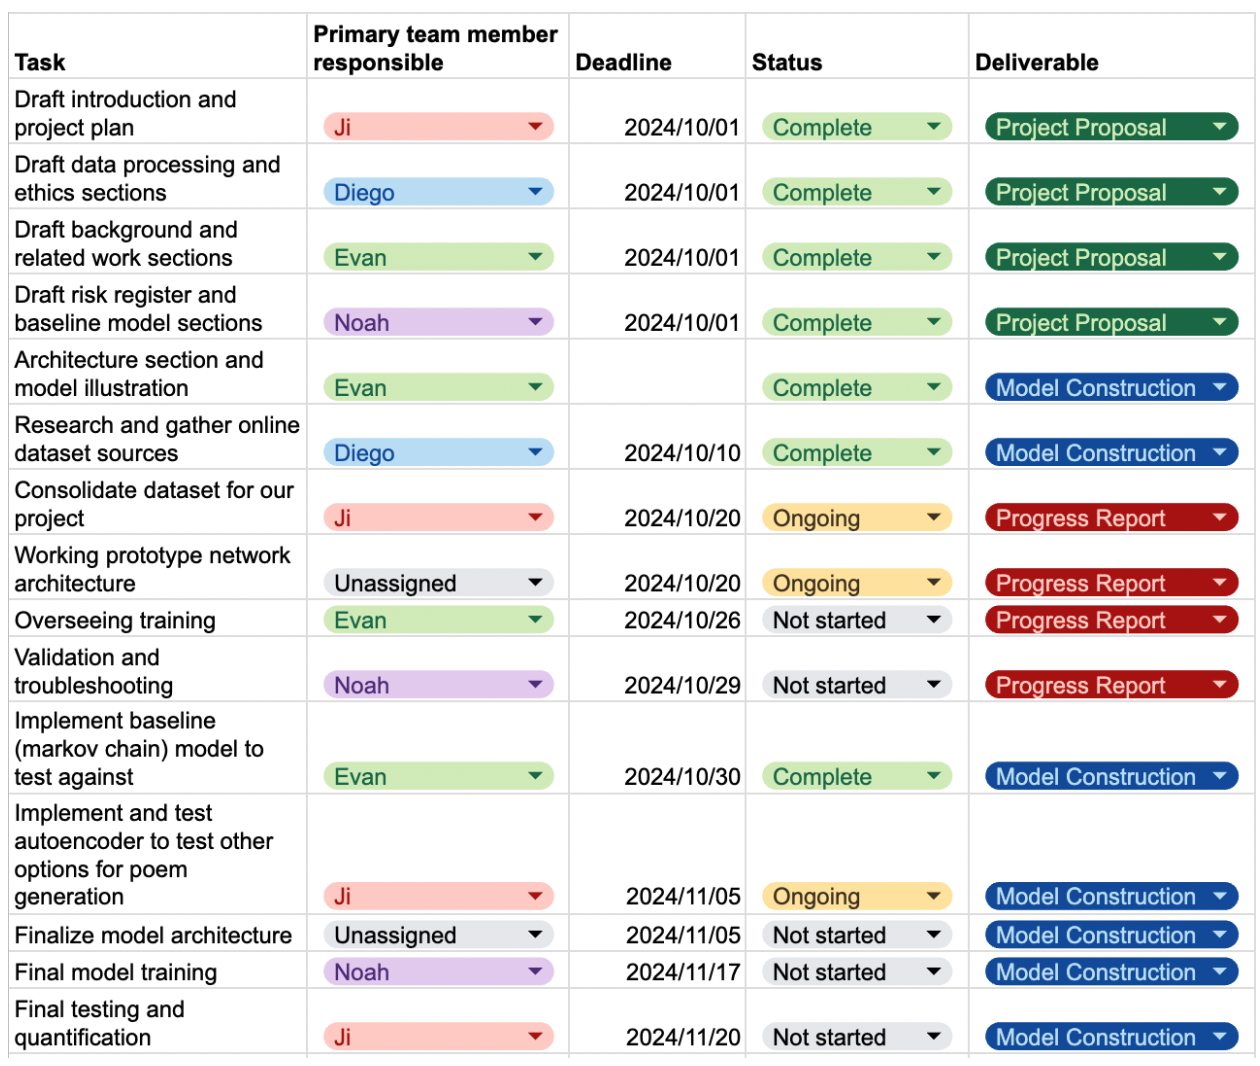
\includegraphics[width=1\textwidth]{Figs/tasktracker.png}
%   \end{center}
%   \caption{Updated Task Tracker}
%   \label{fig:tasktracker}
% \end{figure}

% \begin{figure}[h]
%   \begin{center}
%   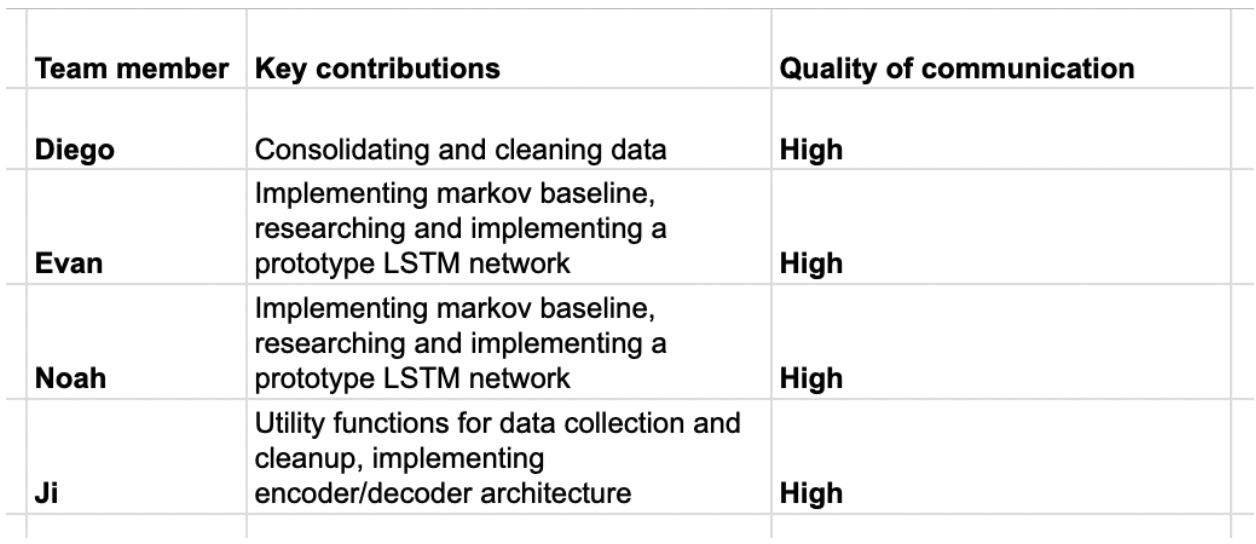
\includegraphics[width=1\textwidth]{Figs/commstable.png}
%   \end{center}
%   \caption{Team communication and contributions}
%   \label{fig:commstable}
% \end{figure}

\section{Notable Contribution}

\subsection{Data Processing}
The main data used for this project consists of the Gutenberg Poetry Corpus dataset in
github \citep{gutenberg_dataset}.
This dataset is publicly available and comes from a web scraper run in 2018.
The web scraper collected poems from the Gutenberg Project, and online repository for public domain literature.
The data comes in the form of a JSON file which has the following fields:
"s", a line of poetry, and "gid" an id of the book in the gutemberg project database.
To clean the data we stripped every line of the poem, and segmented them into "poems" of 10 lines.
We decided to split the data every 10 lines since the main reason for using this data set is to draw from more historical and poetic languge.
Therefore, the actual length of the text we trained our model on is not as relevant since we work out the structure of the haiku through the training.

Another data source we used is the CMU pronouncing dictionary \citep{cmu_pronouncing_dictionary}.
We use this dictionary to count the amount of syllables in each line of the haiku.
Given that this is an open source project with a python library, data cleanup was minimal for this dataset.


After downloading the data, the cleaning process for the haiku dataset consists is run by a python script.
This python script takes in each line of the JSON file, and removes uncommon characters such as the return-carriage character (\texttt{\textbackslash r}), tabs (\texttt{\textbackslash t}), and em-dashes (—).
Next it converts all the characters to lowercase.
And finally, it appends the haiku to a text file in which the end of a poem section is denoted by two new line characters.
The text file is then used at training when loading the data.
Below is an example of the raw input data, and its processed form.



\begin{multicols}{2}

  \textbf{Original (Raw text):} \par
\{ "s": "That was our bench the time you said to me", "gid": "442" \} \\
\{ "s": "The long new poem--but how different now,", "gid": "442" \} \\
\{ "s": "How eerie with the curtain of the fog", "gid": "442" \} \\
\{ "s": "Making it strange to all the friendly trees!", "gid": "442" \} \\
\{ "s": "There is no wind, and yet great curving scrolls", "gid": "442" \} \\
\{ "s": "Carve themselves, ever changing, in the mist.", "gid": "442" \} \\
\{ "s": "Walk on a little, let me stand here watching", "gid": "442" \} \\
\{ "s": "To see you, too, grown strange to me and far. . . .", "gid": "442" \} \\
\{ "s": "I used to wonder how the park would be", "gid": "442" \} \\
\{ "s": "If one night we could have it all alone--", "gid": "442" \} \\

  \columnbreak

  \raggedleft
  \textbf{Finalized (After cleaning):} \par

  \raggedleft
That was our bench the time you said to me \\
The long new poem but how different now \\
How eerie with the curtain of the fog \\
Making it strange to all the friendly trees \\
There is no wind, and yet great curving scrolls \\
Carve themselves, ever changing, in the mist \\
Walk on a little, let me stand here watching \\
To see you, too, grown strange to me and far \\
I used to wonder how the park would be \\
If one night we could have it all alone


\end{multicols}

Another use of the data is in building the vocabulary before training.
To do this we run the entirety of the text file word-by-word into a python dictionary that maps each word to an index.
This lets us represent the words encountered in a numeric form that is easier to deal with.
Finally, we must say that because the nature of this project is generative,
testing new data simply means prompting the model differently.
In adition to being the largest collection of poems we could find,
this data set provides the additional benefit of having a wide range of styles.
This allows us to make more diverse poems as seen below in the qualitative results section.

\section{Architecture}

For our final model, we switched to a neural network centred around the gated recurrent unit (GRU) architecture, which replaced our previous long-short term memory (LSTM) architecture. 
The gated recurrent unit has been shown to be similar to the LSTM architecture on performance and quality of output, while requiring less compute resources during training \citep{LSTMvGRU}, which
appeared to hold true when testing our model and comparing to our previous design. 

%Figure~\ref{fig:flowchart} flowchart.

\begin{figure}[h]
  \begin{center}
  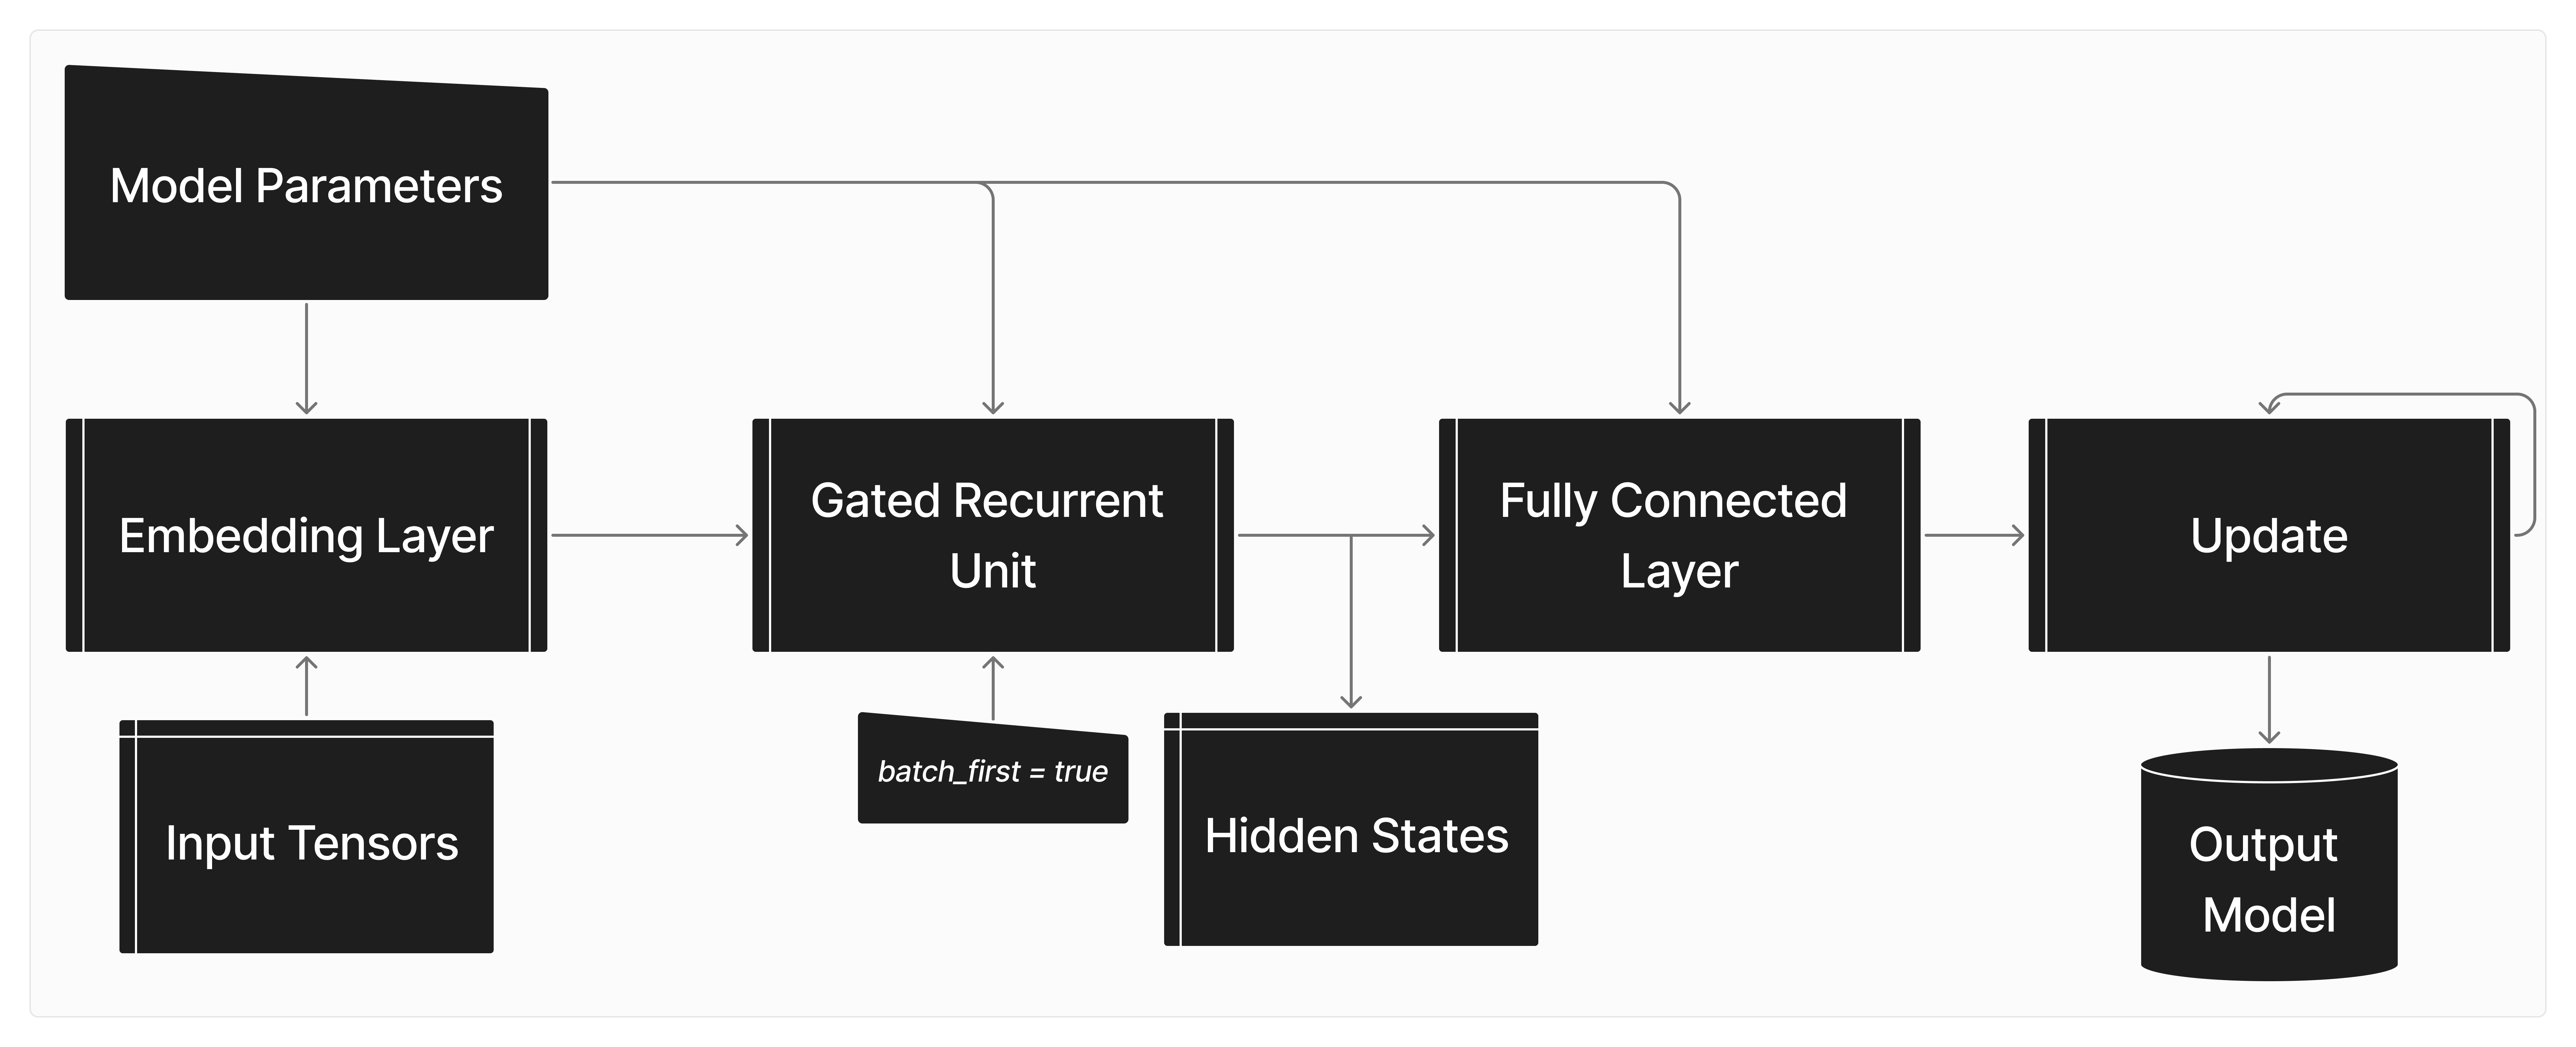
\includegraphics[width=1\textwidth]{Figs/Haiku-Generation.png}
  \end{center}
  \caption{Model Architecture}
  \label{fig:flowchart}
\end{figure}

The architecture of the model is as follows, as described in the Figure~\ref{fig:flowchart} flowchart.

Firstly, the model parameters are manually configured. These include the following, with the hyperparameters we found to work best with our dataset:

\begin{enumerate}
  \item The size of the vocabulary dictionary - which was 109976 distinct words for our data
  \item Embedding dimensions - 128 was found to work well
  \item The index of the padding token within the vocabulary dictionary
  \item The number of hidden dimensions - set to 256
  \item The number of GRU layers - set to 3
  \item How much dropout to apply between layers - we did not use any
  \item If the GRU will perform bidirectional passes - we did not perform these passes
\end{enumerate}

When data is passed to the model, it first goes though the embedding layer. This layer serves to transform this data into vector representations that capture the relationships between words throughout the data. 
The layer takes in the number of unique words in the dataset, the size of the embedding dimension, and the padding token index so that it does not contribute to gradients when training.

The output of that layer is then passed to the Gated Recurrent Unit layer, which serves to
process the sequence of embeddings to capture contextual information across words. It takes in the embedding dimensions, the hidden dimensions, 
the number of GRU layers to have, batch\_first (which should always be set to true for our data),
how much dropout to apply, and if the GRU will perform bidirectional passes. The resulting output of this layer are two tensors, 
one with the output features from the GRU, and another that has the hidden states of the GRU for each layer.

Finally, the output features are passed to a linear layer, which maps them as logits to each word in the vocabulary set. The input size to the layer is the number of input features, 
which is the size of the hidden dimension, and the output size is the number of output features, equal to the size of the vocabulary set.

It should be noted that if the GRU is to perform bidirectional passes, the number of hidden dimensions must be multiplied by two in order to align with the required tensor size.

This model can then be passed to train, for which we used Cross Entropy Loss criterion with the padding index passed as a parameter to ensure it does not contribute to gradients, 
and the Adaptive Movement Estimation (Adam) optimizer. Additionally, we used a learning rate of 0.001, a batch size of 64, and 50 epochs.

\section{Baseline Model}

Our first main baseline model is a markov chain of depth four. This was trained on the same data used in the primary model.
The main structure is shown in figure 0:

\begin{figure}[h]
  \begin{center}
  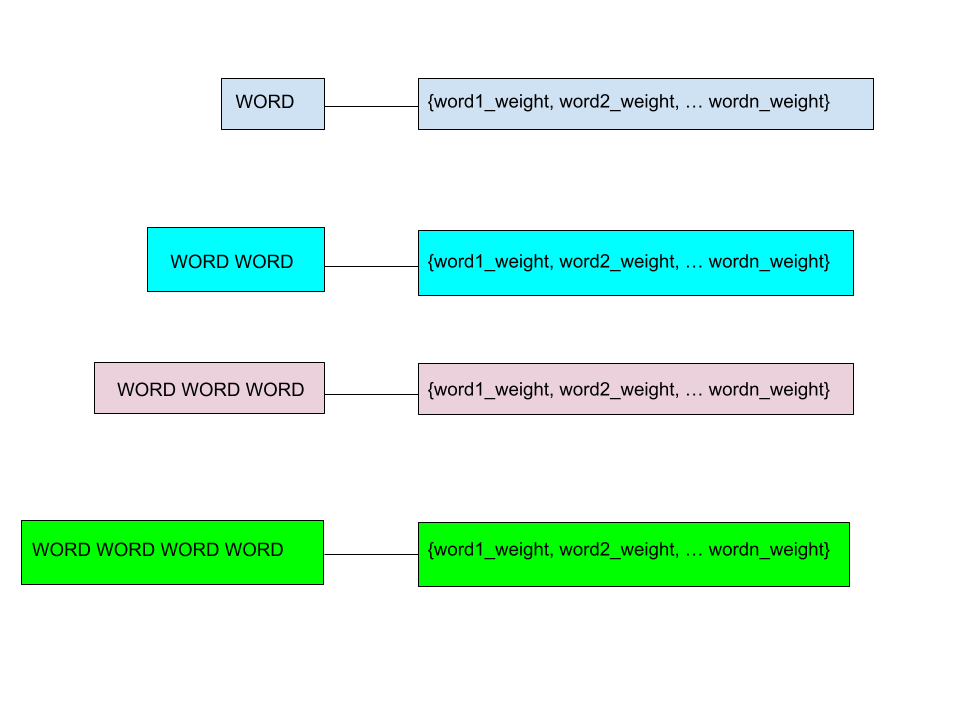
\includegraphics[width=1\textwidth]{Figs/MARKOV.png}
  \end{center}
  \caption{general weighting scheme for markov chain}
  \label{fig:plot}
  \end{figure}

Each individual word in the corpora is assigned a weighting scheme for every word (including itself) based on how frequently those other words come
after the first word.\\
Then every pair of words is assigned a weighting scheme for every word in the corpora based on how likely the word appears after the pair.\\
Then every triple of words is assigned a similar weighting scheme.\\
This repeats until you have a weighting scheme for every n-gram sequence of words up to the depth provided by the function.\\

Throughout this process we treated newline characters and "end of poem" lines (EOP) as distinct words. The model would take in a starting string of
words and would try to autocomplete the poem. It chose words by taking a weighted random choiced based on the weights calculated for the markov
datastructure\\

We chose to use a depth of 4 because lower depths had far more incoherent outputs while higher depths seemed to either return no output
or just directly copy poems for the most part. Here are some example inputs, and their corresponding outputs:\\


Show me:
\begin{flushleft}
  \textit{
      \hspace{2em} show me a garden that's \\
      \hspace{2em} bursting into life
  }
\end{flushleft}

Give:
\begin{flushleft}
  \textit{
      \hspace{2em} give your \\
      \hspace{2em} puppies a little extra\\
      \hspace{2em} thankful that god took me out\\
      \hspace{2em} this funny as hell\\
      \hspace{2em} steve's hair evolving\\
  }
\end{flushleft}


 Teach:
 \begin{flushleft}
  \textit{
      \hspace{2em} teach people  \\
      \hspace{2em} how to get folder icons\\
      \hspace{2em} to show in snowboard\\
  }
\end{flushleft}

It should be noted that these poems were hand-chosen from the markov chain for being more coherent. Often, the markov chain will simply copy
off another poem, return no output, or only return a couple of words, such as the input "teach" generating the output "teach great place to live".\\

Even in the best case, this model struggles to correctly write lines with the correct number of syllables.

We created another baseline model from a very simple LSTM RNN. the structure for this one was a much simpler version of our primary model.\\

It had a 128 dimensional embedding scheme with 2 hidden layers of dimension 256 and a learning rate of 0.001. It was trained with a batch size of 64
for 30 epochs. The output was mostly incoherent so we decided to use the Markov chain as a baseline. All the source code for the first RNN and the
Markov chain is on github, under the jupyter notebook \texttt{RNN\_Model\_1}.


\section{Quantitative Results}

We tested out model with 300 one or two word prompts to the model, and counted the syllables in the output haiku.

\begin{figure}[h]
  \begin{center}
  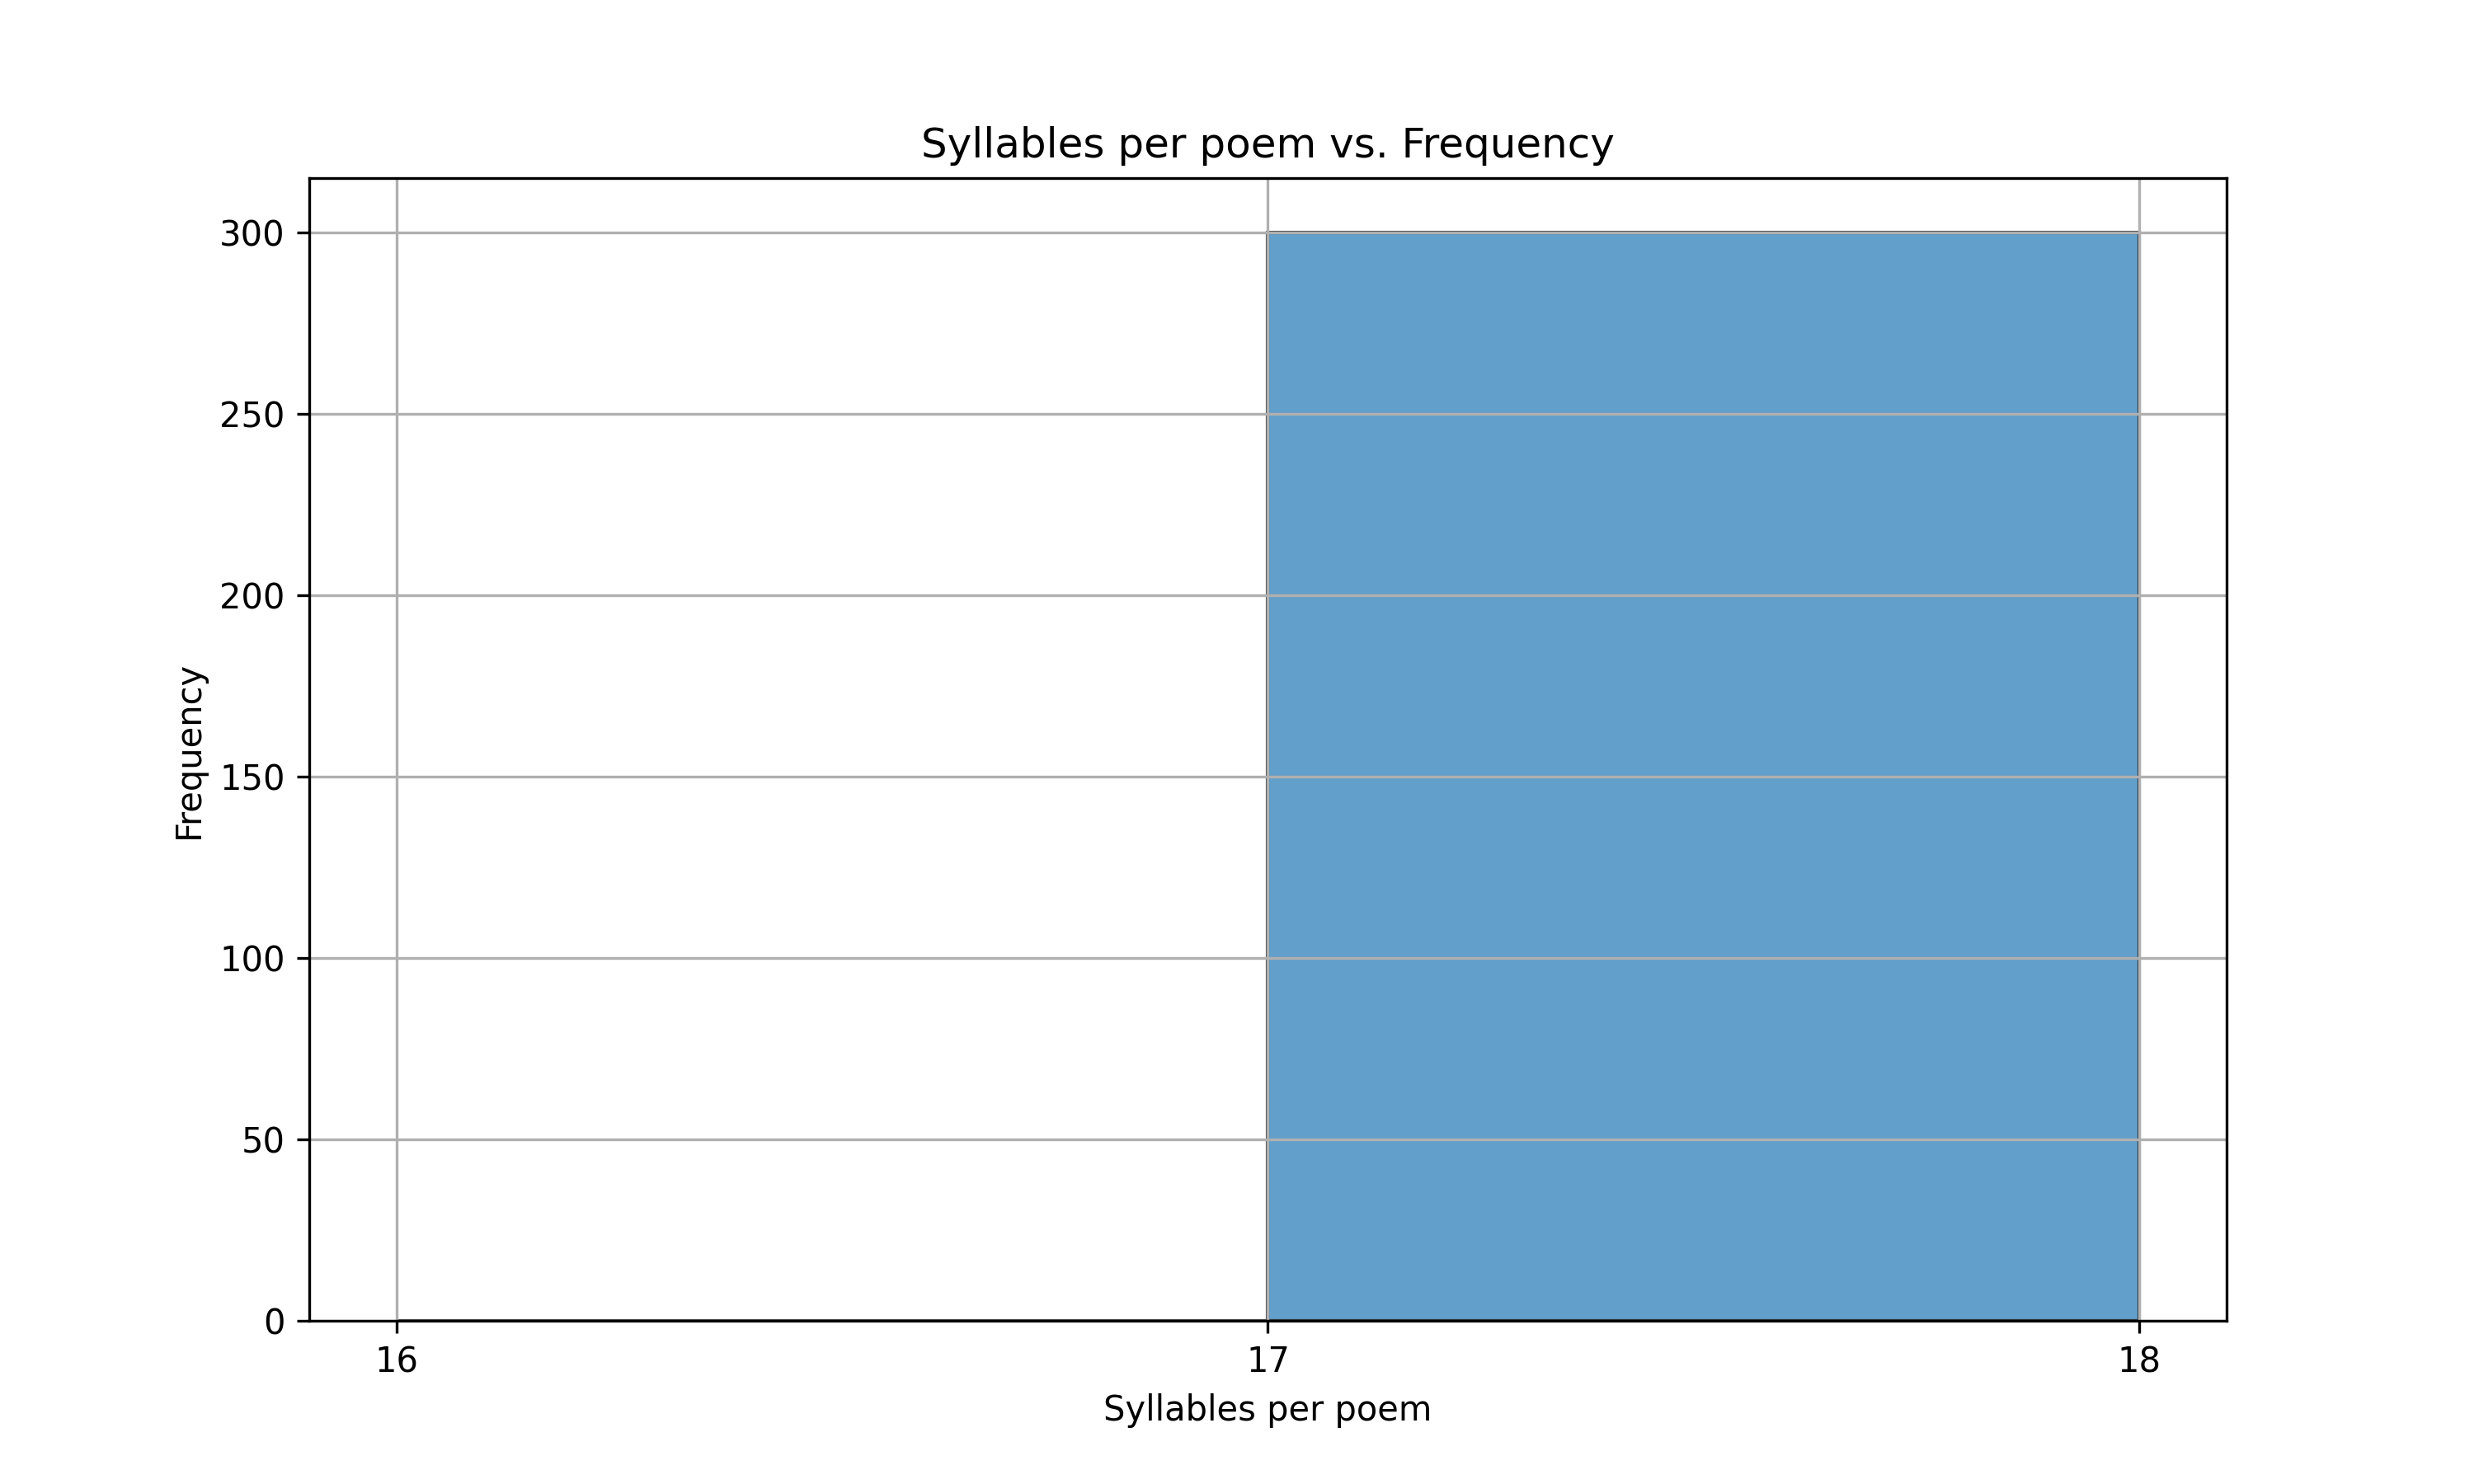
\includegraphics[width=1\textwidth]{Figs/syllable_count_last_word-1.png}
  \end{center}
  \caption{Syllables per haiku from 300 outputs}
  \label{fig:plot1}
\end{figure}

\begin{figure}[h]
  \begin{center}
  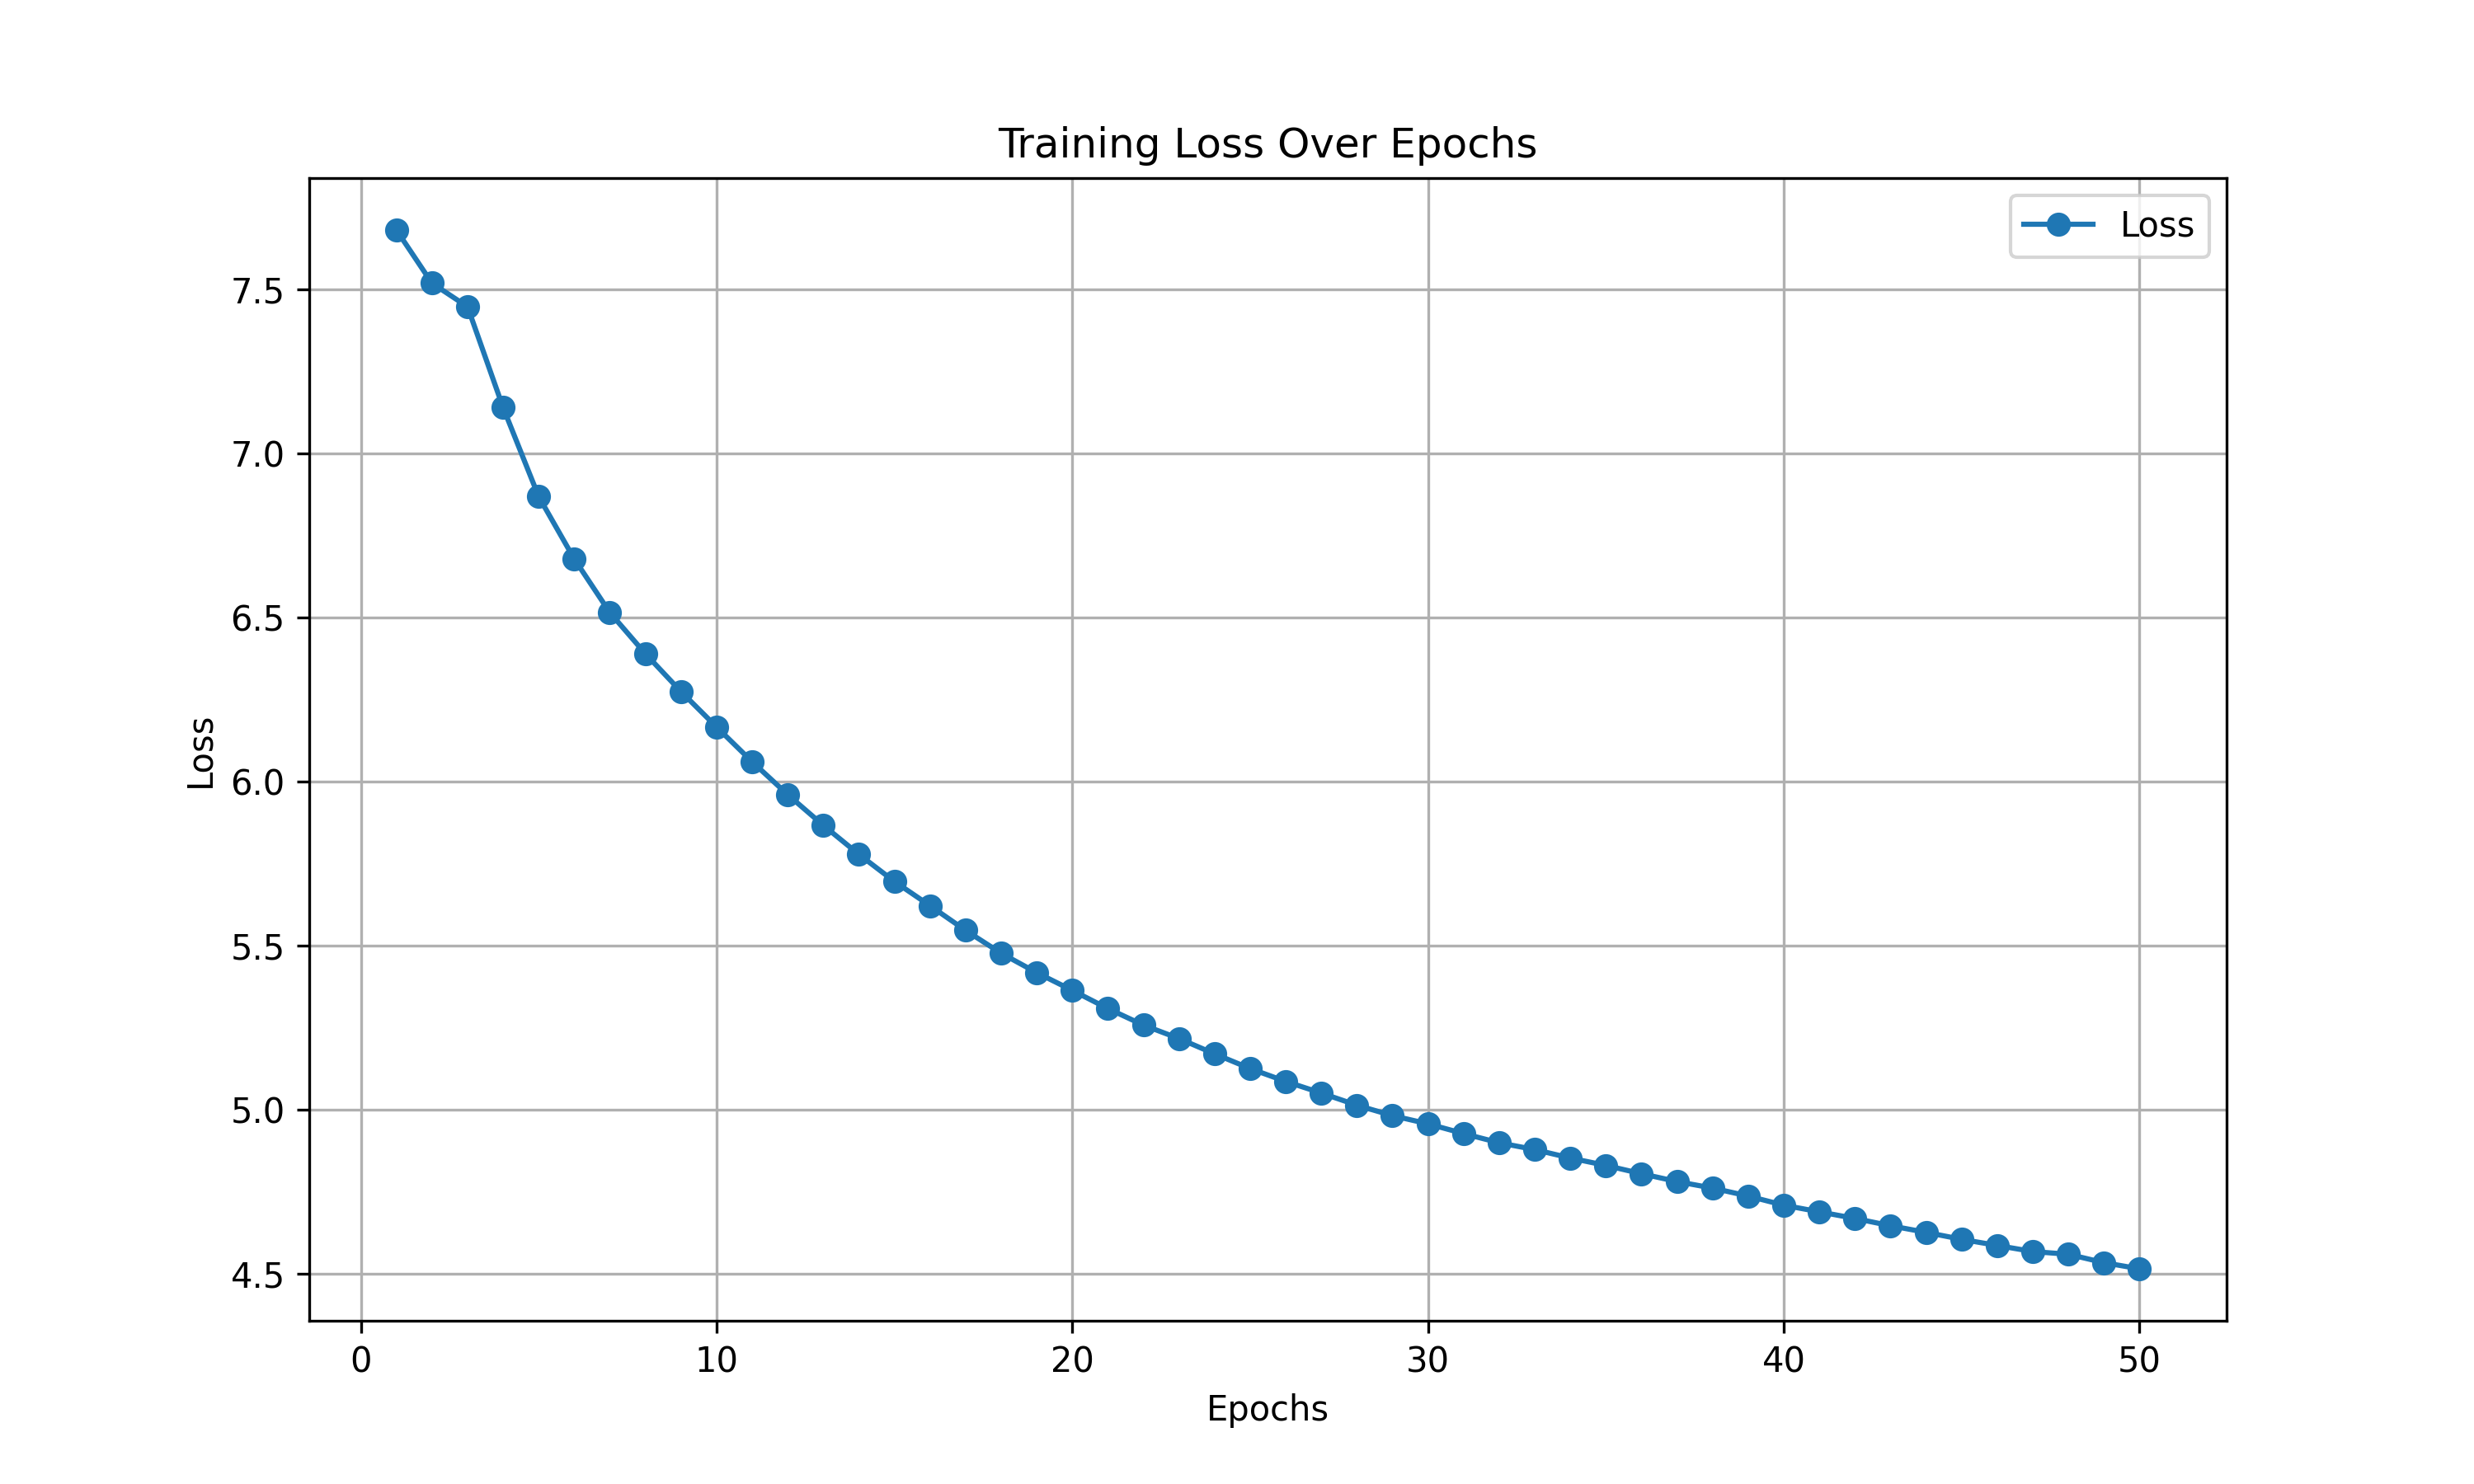
\includegraphics[width=1\textwidth]{Figs/loss-vs-epochs-2.png}
  \end{center}
  \caption{Training Loss over 50 Epochs}
  \label{fig:lossvepochs}
\end{figure}

As shown in Figure~\ref{fig:plot1}, all haikus that were generated by the model meet the 17 syllable count, 
demonstrating the model’s ability to regenerate words dynamically in order to maintain the traditional haiku structure - which was one of the targets from our previous model iteration.

During training, the loss and the rate of loss steadily decreases over the epochs as seen in Figure~\ref{fig:lossvepochs}, showing our model is continuing to learn the meanings of words relative to their neigbours in sentences. 
The loss is calculated as the rate of accuracy between the model's prediction of the next word in a sequence and the original word in that sequence, which reached 4.5 after 50 epochs.

\section{Qualitative Results}
The model generates a mix of interesting or funny hakius, and incoherent outputs:
\begin{itemize}


  \item \textit{"river as thou fledst \\
  she glows within thy dreams where \\
  babe sad favorite"}

  \item \textit{"water from the breeze \\
  there love dejected lies not \\
  here and could he dream"}

  \item \textit{"grass and the moon is \\
  the smoke of a broken tree \\
  is great for the sun"}

  \item \textit{"ocean says she has \\
  to stir stainless nightingale \\
  but well they judge me”}

  \item \textit{“car wolves reach of sighs \\
  and coat an hurrah like strife \\
  truest mother round”}

  \item \textit{“long does fairer by \\
  their heart yet cracks and half so \\
  late they bent him off”}

  \item \textit{“when the death is no \\
  knight ere for my dower and the \\
  vine and hints of that”}

  \item \textit{"wake when spite of love \\
  when that their light are red and \\
  many a star sweet”}

\end{itemize}

As we can see, the model is able to generate haikus that could pass for human-written, however, it still generates
incoherent haikus.
While the decision to make train the haikus in poetry rather than haikus resulted in more poetic language,
it also increased the frequency of rarely used words.

The main challenges we faced making this model were
related to ensuring syllable structure and was maintained and the syllable counts were accurate, and
slow training times.

Because of irregularities in the English Language, we found it difficult to
come up with a reliable method to count the number of syllables in a given word. Our current solution involves referencing
the CMU Pronouncing Dictionary \citep{cmu_pronouncing_dictionary} to get the syllable count of a given word.
However, this method is not perfect, as the CMU Pronouncing Dictionary does not contain all words that may show up in our vocabulary.
This causes issues when a word is not in the dictionary, so we opted for heuristic algorithms to fix this,
although this is still not perfect in practice, it significantly reduced the number of times the 5-7-5 meter was broken.

Despite gaining more resources for training through Vertex AI,
this is not a sustainable way of training the model as it quickly runs out of free compute credits.
However, using even just the free Tier drastically increased the speed at which we were able to train the model.

\section{Evaluation on new data}
To evaluate our model, we generated dozens of new poems from varying inputs and chose the five that we believed were the most coherent to represent the model. We then created a survey with 15 poems. These consisted of the 5 made by our model, 5 chosen from the more coherent outputs of the baseline markov chain, and 5 chosen from the repository of human written poems that we used in training. We had 24 people rate the quality of each poem from 1 to 10, and averaged all the responses. The results are shown in the figure below:

\begin{figure}[h]
  \begin{center}
  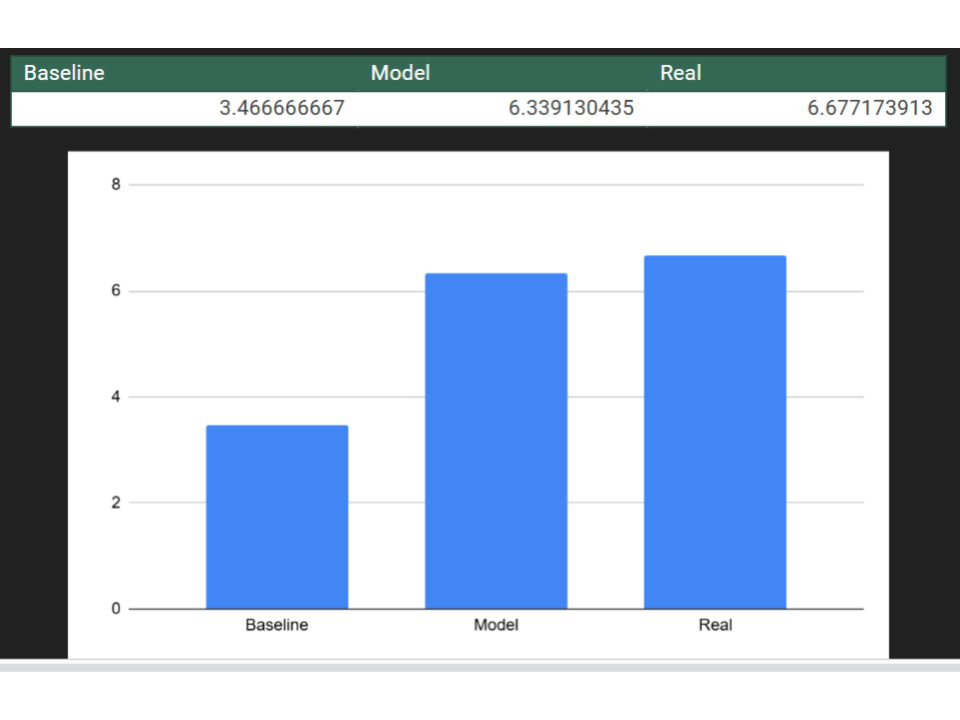
\includegraphics[width=1\textwidth]{Figs/survey_results.png}
  \end{center}
  \caption{Syllables per haiku from 300 outputs}
  \label{fig:plot2}
\end{figure}
\FloatBarrier

the five poems used in the survey from our model are:

\begin{itemize}


  \item \textit{"winter chill with hopes \\
  of peace they see the home to \\
  sleep and we are heard"}

  \item \textit{"new grass like diamonds \\
  blowing through the darker sounds \\
  of heaven to flame"}

  \item \textit{"the mightiest makes \\
  the memory of some three \\
  shepherds from the glow"}

  \item \textit{"the charm of his heart \\
  the graceful hills of the brow \\
  and the black essence}

  \item \textit{the ravenous sand \\
  the graveyard for the raindrops \\
  and the gothic feet}

\end{itemize}

\section{Ethical Considerations}

Despite AI being around for several decades, it was only recently that computational power necessary to generate human-level works of art became widely available.
As impressive as they are, Increasingly improving models that generate images, written stories, and poems also raise questions about how these models get and utilize their training data.
While this is a very trending topic, legislation protecting individuals from having their written works used to train AI models is still in early stages.
Because of this we have decided to only use works in the public domain.
The works we use in this model can all be found in the Gutemberg Project digital library meaning none of them are held under exclusive rights.
Finally, this model is a purely academic experiment, and we do not seek to benefit from the material it generates.
Therefore, the literary works we will deal with in this project and our use of them fall under fair dealings as per Canadian law \citep{LegislativeServicesBranch_2024} .

We have discussed the steps that we will take to prevent misuse of our training data, now let's dig deeper into how someone with harmful intentions might use our project.
The biggest cause of concern comes from poem-writing competitions.
Instead of having to naturally come up with poems, someone might take advantage of a deep learning model to easily generate several entries, increasing their chances of winning or simply overloading the contest's submission portal.
While many competitions may not explicitly ban AI-generated poems, it is not hard to see how a generated poem winning over many human authors may be seen as controversial.
Our system somewhat counteracts this by having the user be vital in the poem creation as they must prompt the model in order for it to generate anything.
Additionally, our limited scope of haikus would make it harder for someone to take advantage of the model on a massive scale as haikus are notoriously short.
With these ethical considerations, we can confidently say that misuse of this model his highly unlikey.


%\pagebreak

\newpage
\clearpage

\label{last_page}

\bibliography{APS360_ref}
\bibliographystyle{iclr2022_conference}

\end{document}
